\documentclass{article}
% Choose a conveniently small page size
% PACKAGES
\usepackage[margin = 1in]{geometry}
\usepackage{amsfonts}
\usepackage{amsmath}
\usepackage{amssymb}
\usepackage{multicol}
\usepackage{graphicx}
\usepackage{float}
\usepackage{xcolor}
\usepackage{amsthm}
\usepackage{dsfont}
\usepackage{hyperref}
\usepackage{subcaption}
\usepackage{listings}

\lstset{
  language=Python,
  basicstyle=\ttfamily\small,
  keywordstyle=\color{blue},
  stringstyle=\color{red},
  commentstyle=\color{olive},
  morecomment=[l][\color{magenta}]{\#},
  showstringspaces=false
}

% MACROS
% Set Theory
\def\N{\mathbb{N}}
\def\R{\mathbb{R}}
\def\C{\mathbb{C}}
\def\Z{\mathbb{Z}}
%\def\^{\hat}
\def\-{\vec}
\def\d{\partial}
\def\!{\boldsymbol}
\def\X{\times}
%\def\-{\bar}
\def\bf{\textbf}
\def\l{\left}
\def\r{\right}
\title{Weekly Report}
\author{Damien Beecroft}
\begin{document}
\maketitle
% \newpage
\section{Discretization Methods}
$f$ is a three dimensional tensor with elements $f_{i,j,k}$ that approximates the density of the molecules in the 1D2V phase space. $Q^+(f,f)$ is a three dimensional tensor with elements $Q^+_{i,j,k}(f,f)$ that approximates of the gain term of the collision operator of $f$. $v$ is a matrix with elements $v_{j,k}$ that approximates the velocities that particles can take on. $\rho$ is a vector with elements $\rho_i$ that approximates the spatial density function of the solution. The first dimension of this tensor (indexed by $i$) is the spatial dimension. $i \in \{0,I\}$. The second dimension of this tensor (indexed by $j$) is the first velocity dimension. $j \in \{0,J\}$. The third dimension of this tensor (indexed by $k$) is the first velocity dimension. $k \in \{0,K\}$. In the code implementation we have $I=100$, $J=31$, and $K=31$. All code can be found on my GitHub.
\subsection{Lax-Friedrichs Discretization}
We use $f_i$ as short-hard for $f_{i,*,*}$. We use $Q^+_i(f,f)$ as short-hard for $Q^+_{i,*,*}(f,f)$.  We are implementing the Lax-Friedrichs fast sweeping method for the Boltzmann equation. The left to right sweep is given by
\[
  \frac{v + |v|}{2} \frac{f_i^{(l+1)} - f_{i-1}^{(l+1)}}{\Delta x} + \frac{v - |v|}{2} \frac{f_{i+1}^{(l)} - f_{i}^{(l+1)}}{\Delta x} = Q_i^+(f^{(l)}, f^{(l)}) - C \rho_i^{(l)} f_i^{(l+1)}
\]
and the right to left sweep is given by
\[
  \frac{v + |v|}{2} \frac{f_i^{(l+1)} - f_{i-1}^{(l)}}{\Delta x} + \frac{v - |v|}{2} \frac{f_{i+1}^{(l+1)} - f_{i}^{(l+1)}}{\Delta x} = Q_i^+(f^{(l)}, f^{(l)}) - C \rho_i^{(l)} f_i^{(l+1)}.
\]
These discretizations result in the following update schemes. For left to right we have 
\begin{gather*}
  \frac{v + |v|}{2} \frac{f_i^{(l+1)} - f_{i-1}^{(l+1)}}{\Delta x} + \frac{v - |v|}{2} \frac{f_{i+1}^{(l)} - f_{i}^{(l+1)}}{\Delta x} = Q_i^+(f^{(l)}, f^{(l)}) - C \rho_i^{(l)} f_i^{(l+1)} \to \\
  \frac{v + |v|}{2 \Delta x} f_{i}^{(l+1)} - \frac{v + |v|}{2 \Delta x} f_{i-1}^{(l+1)} + \frac{v - |v|}{2 \Delta x} f_{i+1}^{(l)} - \frac{v - |v|}{2 \Delta x} f_{i}^{(l+1)} = Q_i^+(f^{(l)}, f^{(l)}) - C \rho_i^{(l)} f_i^{(l+1)} \to \\
  \frac{v + |v|}{2 \Delta x} f_{i}^{(l+1)} - \frac{v - |v|}{2 \Delta x} f_{i}^{(l+1)} = Q_i^+(f^{(l)}, f^{(l)}) - C \rho_i^{(l)} f_i^{(l+1)} + \frac{v + |v|}{2 \Delta x} f_{i-1}^{(l+1)} - \frac{v - |v|}{2 \Delta x} f_{i+1}^{(l)} \to \\
  \frac{|v|}{\Delta x} f_{i}^{(l+1)} = Q_i^+(f^{(l)}, f^{(l)}) - C \rho_i^{(l)} f_i^{(l+1)} + \frac{v + |v|}{2 \Delta x} f_{i-1}^{(l+1)} - \frac{v - |v|}{2 \Delta x} f_{i+1}^{(l)} \to \\
  \left(\frac{|v|}{\Delta x} + C \rho_i^{(l)} \right) f_{i}^{(l+1)} = Q_i^+(f^{(l)}, f^{(l)}) + \frac{v + |v|}{2 \Delta x} f_{i-1}^{(l+1)} - \frac{v - |v|}{2 \Delta x} f_{i+1}^{(l)} \to \\
  f_{i}^{(l+1)} = \left(\frac{|v|}{\Delta x} + C \rho_i^{(l)} \right)^{-1} \left( Q_i^+(f^{(l)}, f^{(l)}) + \frac{v + |v|}{2 \Delta x} f_{i-1}^{(l+1)} - \frac{v - |v|}{2 \Delta x} f_{i+1}^{(l)} \right).
\end{gather*}
For right to left we then have
\begin{gather*}
  f_{i}^{(l+1)} = \left(\frac{|v|}{\Delta x} + C \rho_i^{(l)} \right)^{-1} \left( Q_i^+(f^{(l)}, f^{(l)}) + \frac{v + |v|}{2 \Delta x} f_{i-1}^{(l)} - \frac{v - |v|}{2 \Delta x} f_{i+1}^{(l+1)} \right).
\end{gather*}

\subsection{Time Stepping Discretization}
This is a simple advection scheme with the the added complication that each $v_{j,k}$ may be positive or negative. We must consider cases where $0 < v_{j,k}$ separately from cases where $0 > v_{j,k}$ because these slices of the molecules in the phase space are advecting in different directions. We first focus on the right advecting part of the equation. For the following equation let $f_i$ be short-hand for all $f_{i,j,k}$ such that $0 < v_{j,k}$. Let $v_+$ be short-hand for all $v_{j,k}$ such that $0 < v_{j,k}$.
\begin{gather*}
  \frac{f_i^* - f_i^{(l)}}{\Delta t} + v_+ \frac{f_i^{(l)} - f_{i-1}^{(l+1)}}{\Delta x} = 0\\
  \frac{f_i^{(l+1)} - f^*_i}{\Delta t} = Q_i^+(f^*,f^*) - C \rho_i^* f^*_i.
\end{gather*}
This results in the following update scheme.
\begin{gather*}
  f_i^* = f_i^{(l)} - \frac{v_+ \Delta t}{\Delta x} \left( f_i^{(l)} - f_{i-1}^{(l+1)} \right)\\
  f_i^{(l+1)} = f^*_i + \Delta t \left( Q_i^+(f^*,f^*) - C \rho_i^* f^*_i \right).
\end{gather*}
Now, we focus on the left advecting part of the equation. For the following equation let $f_i$ be short-hand for all $f_{i,j,k}$ such that $0 > v_{j,k}$. Let $v_-$ be short-hand for all $v_{j,k}$ such that $0 > v_{j,k}$.
\begin{gather*}
  \frac{f_i^* - f_i^{(l)}}{\Delta t} + v_- \frac{f_{i+1}^{(l+1)} - f_{i}^{(l)}}{\Delta x} = 0\\
  \frac{f_i^{(l+1)} - f^*_i}{\Delta t} = Q_i^+(f^*,f^*) - C \rho_i^* f^*_i.
\end{gather*}
This results in the following update scheme.
\begin{gather*}
  f_i^* = f_i^{(l)} - \frac{v_- \Delta t}{\Delta x} \left( f_{i+1}^{(l+1)} - f_{i}^{(l)} \right)\\
  f_i^{(l+1)} = f^*_i + \Delta t \left( Q_i^+(f^*,f^*) - C \rho_i^* f^*_i \right).
\end{gather*}
\subsubsection{Boundary Conditions}
Again, the boundary conditions for this method are slightly complicated due to the fact that positive and negative advection velocities are present in the equation. Let Consider a 1D slice of $f$: $f_{*,j,k}$. If $0 < v_{j,k}$, then information is advecting from left to right. For these cases we set Dirichlet boundary conditions on the left. For the normal shock problem the left BC is $\lim_{x \to -\infty} f := f_L$. We do not set boundary conditions on the right. We simply let the flow advect out of the domain. If $0 > v_{j,k}$, then information is advecting from right to left. For these cases we set Dirichlet boundary conditions on the right. For the normal shock problem the right BC is $\lim_{x \to \infty} f = f_R$. We do not set boundary conditions on the left. We simply let the flow advect out of the domain.
\section{Time Stepping Results}
\begin{figure}[H]
  \centering
  \begin{subfigure}[b]{\textwidth}
  \includegraphics[width=\textwidth]{imgs/time_step/output_implicit/0.png}
      % \caption{Image 1}
      \label{fig:image1}
  \end{subfigure}
  \hfill
  \begin{subfigure}[b]{\textwidth}
  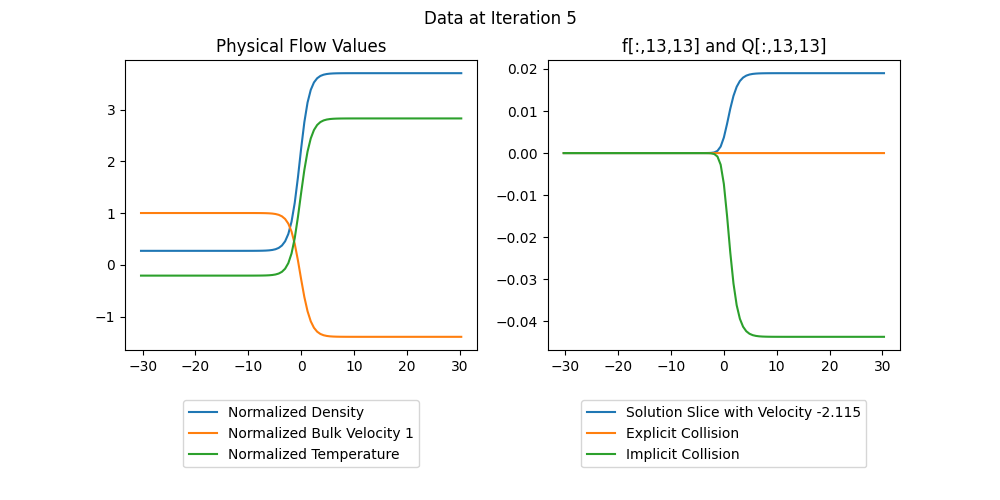
\includegraphics[width=\textwidth]{imgs/time_step/output_implicit/5.png}
      % \caption{Image 2}
      \label{fig:image2}
  \end{subfigure}
\end{figure}
  
\begin{figure}[H]
  
  \begin{subfigure}[b]{\textwidth}
  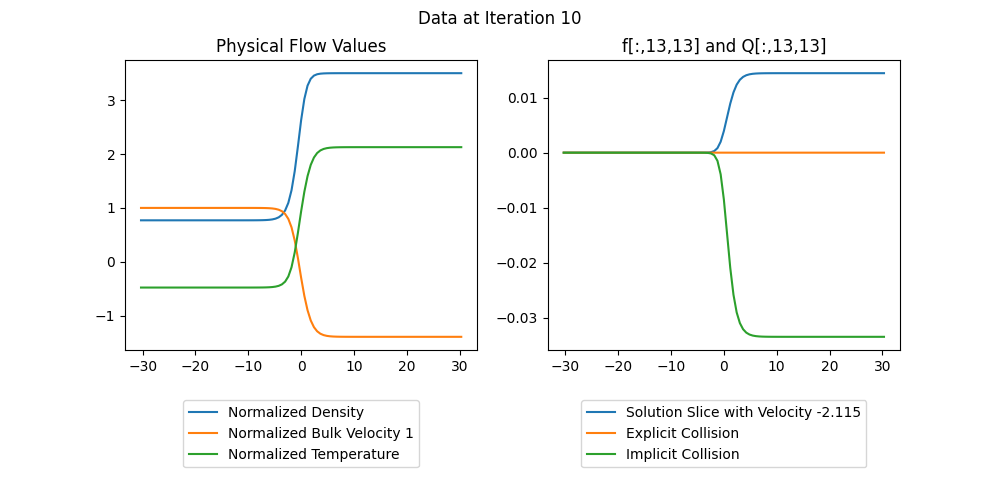
\includegraphics[width=\textwidth]{imgs/time_step/output_implicit/10.png}
      % \caption{Image 3}
      \label{fig:image3}
  \end{subfigure}
  \hfill
  \begin{subfigure}[b]{\textwidth}
  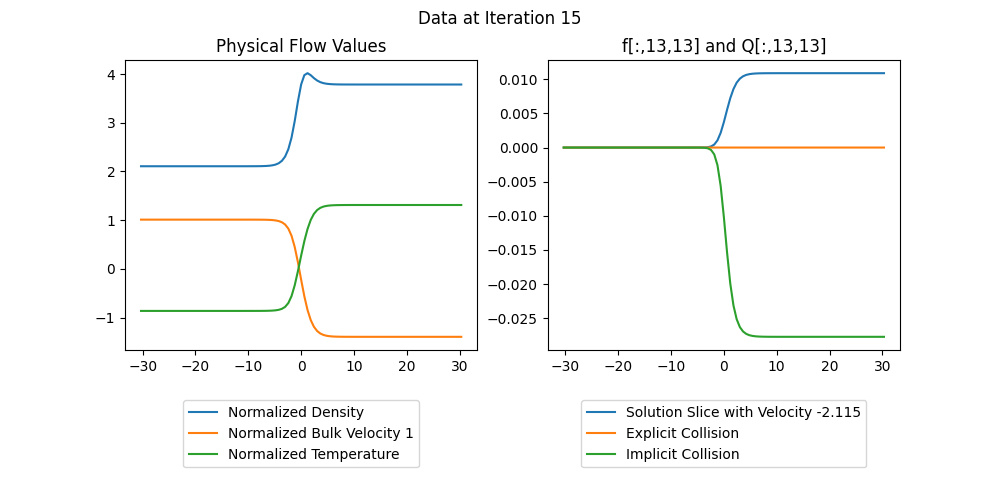
\includegraphics[width=\textwidth]{imgs/time_step/output_implicit/15.png}
      % \caption{Image 4}
      \label{fig:image4}
  \end{subfigure}
\end{figure}

\subsubsection{Explicit Time-Stepping}

\begin{figure}[H]
  \centering
  \begin{subfigure}[b]{\textwidth}
  \includegraphics[width=\textwidth]{imgs/time_step/output_explicit/0.png}
      % \caption{Image 1}
      % \label{fig:image1}
  \end{subfigure}
  \hfill
  \begin{subfigure}[b]{\textwidth}
  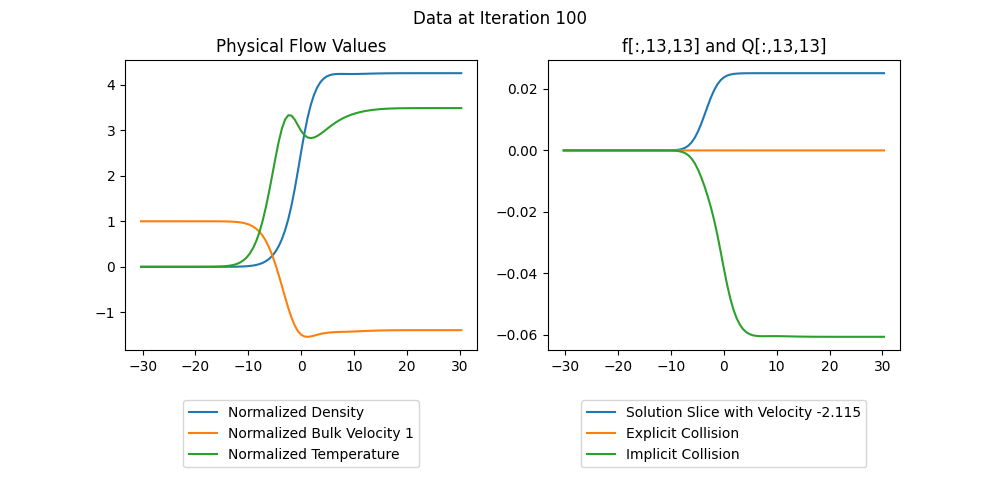
\includegraphics[width=\textwidth]{imgs/time_step/output_explicit/100.png}
      % \caption{Image 2}
      % \label{fig:image2}
  \end{subfigure}
\end{figure}
  
\begin{figure}[H]
  
  \begin{subfigure}[b]{\textwidth}
  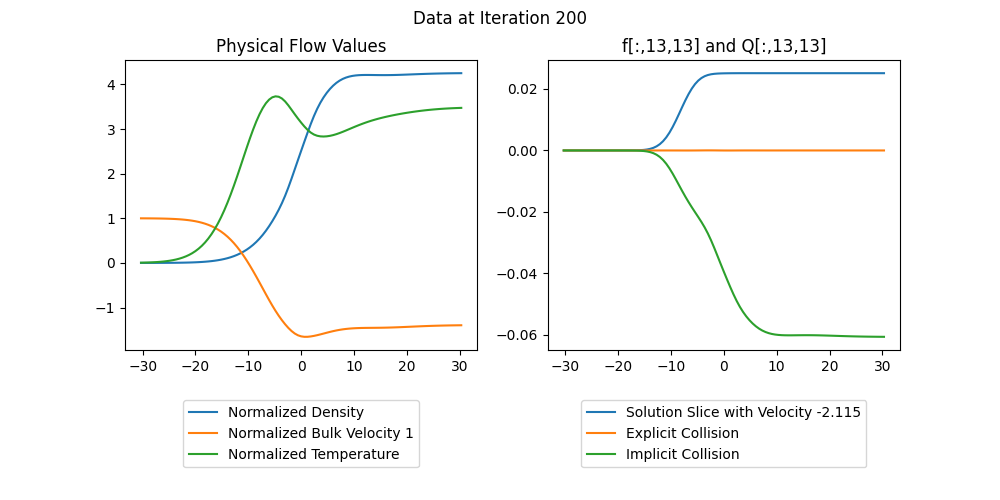
\includegraphics[width=\textwidth]{imgs/time_step/output_explicit/200.png}
      % \caption{Image 3}
      % \label{fig:image3}
  \end{subfigure}
  \hfill
  \begin{subfigure}[b]{\textwidth}
  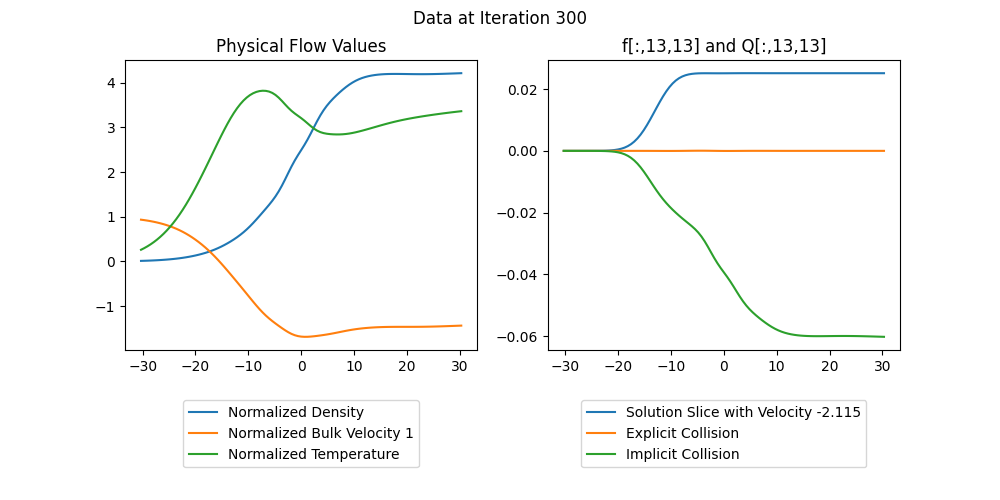
\includegraphics[width=\textwidth]{imgs/time_step/output_explicit/300.png}
      % \caption{Image 4}
      % \label{fig:image4}
  \end{subfigure}
\end{figure}
\subsubsection{Implicit Lax-Friedrichs}
\begin{figure}[H]
  \centering
  \begin{subfigure}[b]{\textwidth}
  \includegraphics[width=\textwidth]{imgs/lax_friedrichs/output_implicit/0.png}
      % \caption{Image 1}
      % \label{fig:image1}
  \end{subfigure}
  \hfill
  \begin{subfigure}[b]{\textwidth}
  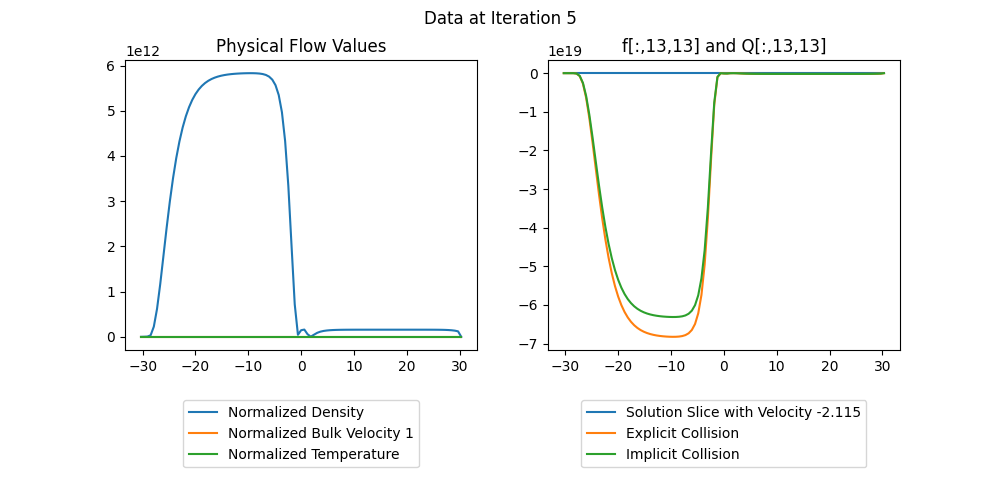
\includegraphics[width=\textwidth]{imgs/lax_friedrichs/output_implicit/5.png}
      % \caption{Image 2}
      % \label{fig:image2}
  \end{subfigure}
\end{figure}
  
\begin{figure}[H]
  
  \begin{subfigure}[b]{\textwidth}
  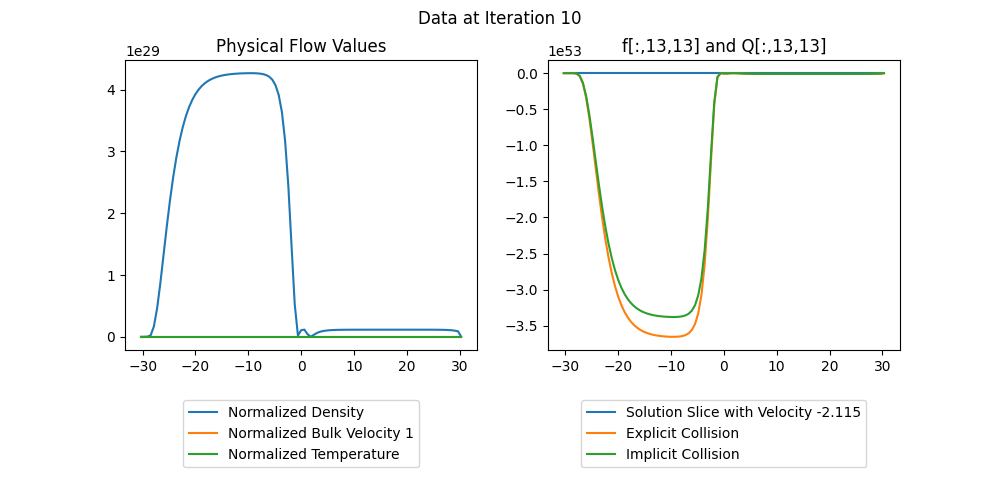
\includegraphics[width=\textwidth]{imgs/lax_friedrichs/output_implicit/10.png}
      % \caption{Image 3}
      % \label{fig:image3}
  \end{subfigure}
  \hfill
  \begin{subfigure}[b]{\textwidth}
  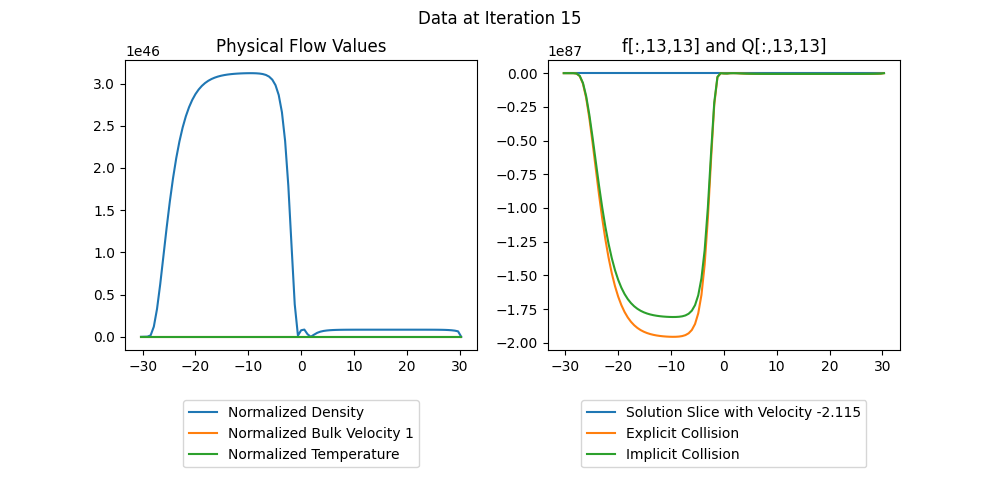
\includegraphics[width=\textwidth]{imgs/lax_friedrichs/output_implicit/15.png}
      % \caption{Image 4}
      % \label{fig:image4}
  \end{subfigure}
\end{figure}

\end{document}
% \subsubsection{Boundary Conditions for Lax-Friedrichs Method}
% The boundary conditions for this method are slightly complicated due to the fact that positive and negative advection velocities are present in the equation. Let Consider a 1D slice of $f$: $f_{*,j,k}$. If $0 < v_{j,k}$, then information is advecting from left to right. For these cases we set Dirichlet boundary conditions on the left. For the normal shock problem the left BC is $\lim_{x \to -\infty} f := f_L$. On the right we simply use extrapolation boundary conditions: $f_{I,j,k} = 2f_{I-1,j,k} - f_{I-2,j,k}$. If $0 > v_{j,k}$, then information is advecting from right to left. For these cases we set Dirichlet boundary conditions on the right. For the normal shock problem the right BC is $\lim_{x \to \infty} f = f_R$. On the left we simply use extrapolation boundary conditions: $f_{0,j,k} = 2f_{1,j,k} - f_{2,j,k}$
% \[
%   \frac{v + |v|}{2} \frac{f_i^{(l+1)} - f_{i-1}^{(l+1)}}{\Delta x} + \frac{v - |v|}{2} \frac{f_{i+1}^{(l)} - f_{i}^{(l+1)}}{\Delta x} = Q_i^+(f^{(l)}, f^{(l)}) - C \rho_i^{(l)} f_i^{(l+1)}
% \]

% This is a simple advection scheme with the the added complication that each $v_{j,k}$ may be positive or negative. If $0 < v_{j,k}$, then we set Dirichlet boundary conditions on the left and let $f_{*,j,k}$ advect to the right. We use extrapolation boundary conditions on the right: $2f_{N,j,k} - f_{N-1,j,k} = f_{N+1,j,k}$. Otherwise, if $0 > v_{j,k}$, then we set Dirichlet boundary conditions on the right and let $f_{*,j,k}$ advect to the right. 

% $2f_N - f_{N-1} = f_{N+1}$
% The notation here is a bit fast and loose. In the 1D2V case that we are modeling, each $v$ and $f_\cdot^{(\cdot)}$ is a matrix. This is due to the fact that there is a two dimensional velocity field. So, we end up doing a Hadamard product at every iteration. Anyhow, t

% This 1D slice is the discretized density function over all of $x$ advecting with velocity $v_{j,k}$. 